\chapter{Optimal Aperture by Blur-Percentile Definition}
\label{ch:percentile}

Every earlier blur-optimization chapter used $r_{EE}(50\%)$ as the reported metric.
This chapter asks directly: does the optimal aperture change if a different encircled-energy
percentile is used, and --- since $r_{EE}(50\%)$'s own documentation
(Section~\ref{sec:effective-radius}) flags it as prone to a grid-resolution floor at
well-focused, large-aperture conditions --- is $r_{EE}(50\%)$ actually a trustworthy
metric for this comparison in the first place?

\section{Optimal aperture, four percentiles}

\begin{table}[htbp]
\centering
\begin{tabular}{rrrrr}
\toprule
$M$ (D) & $r_{EE}(50\%)$ optimum & $r_{EE}(70\%)$ optimum & $r_{EE}(80\%)$ optimum & $r_{EE}(90\%)$ optimum \\
\midrule
0 & 700   & 1000  & 1250  & 2000 \\
1 & 700   & 1000  & 1250  & 1250 \\
2 & 750   & 600   & 750   & 1000 \\
3 & 600   & 500   & 750   & 750  \\
4 & 500   & 500   & 600   & 750  \\
5 & 500   & 400   & 600   & 600  \\
6 & 400   & 400   & 500   & 600  \\
8 & 400   & 300   & 400   & 500  \\
\bottomrule
\end{tabular}
\caption{Optimal aperture (\textmu m) by blur-minimization percentile and myopia level.}
\label{tab:percentile-optima}
\end{table}

\section{A saturation artifact, identified and quantified}

Directly inspecting the underlying per-aperture curve at $M=0\,$D reveals why the
$M=0$/$M=1$ rows of Table~\ref{tab:percentile-optima} should not be read at face
value:
\begin{center}
\begin{tabular}{rrrr}
\toprule
$a_{hole}$ & $r_{EE}(50\%)$ & $r_{EE}(70\%)$ & $r_{EE}(80\%)$ \\
\midrule
$700\um$  & $7.328\um$ & $11.07\um$ & $13.69\um$ \\
$1000\um$ & $7.328\um$ & $7.328\um$ & $9.24\um$ \\
$1250\um$ & $7.328\um$ & $7.328\um$ & $7.328\um$ \\
$2000\um$ & $7.328\um$ & $7.328\um$ & $7.328\um$ \\
\bottomrule
\end{tabular}
\end{center}
From aperture $700\um$ through $2000\um$, $r_{EE}(50\%)$, and beyond $1250\um$ even
$r_{EE}(80\%)$, pin to the \emph{exact same} numerical value ($7.327531\um$) rather
than continuing to decrease --- the grid/histogram bin-width floor documented in
Section~\ref{sec:effective-radius}. At $M=0$--$1$, the diffraction-limited spot is
tight enough that several distinct percentiles of encircled energy all collapse onto
this floor simultaneously, at apertures well within the tested range. \textbf{The
reported ``optimal'' aperture for $r_{EE}(70\%)$/$r_{EE}(80\%)$ at these two myopia
levels is therefore an arbitrary pick off a flat plateau, not a genuine unique
minimum.}

For $M\ge2\,$D, this issue is absent: the underlying per-aperture curves are clean,
well-resolved U-shapes with no ties at any tested percentile, and the corresponding
rows of Table~\ref{tab:percentile-optima} are genuine, trustworthy optima.

\begin{figure}[htbp]
\centering
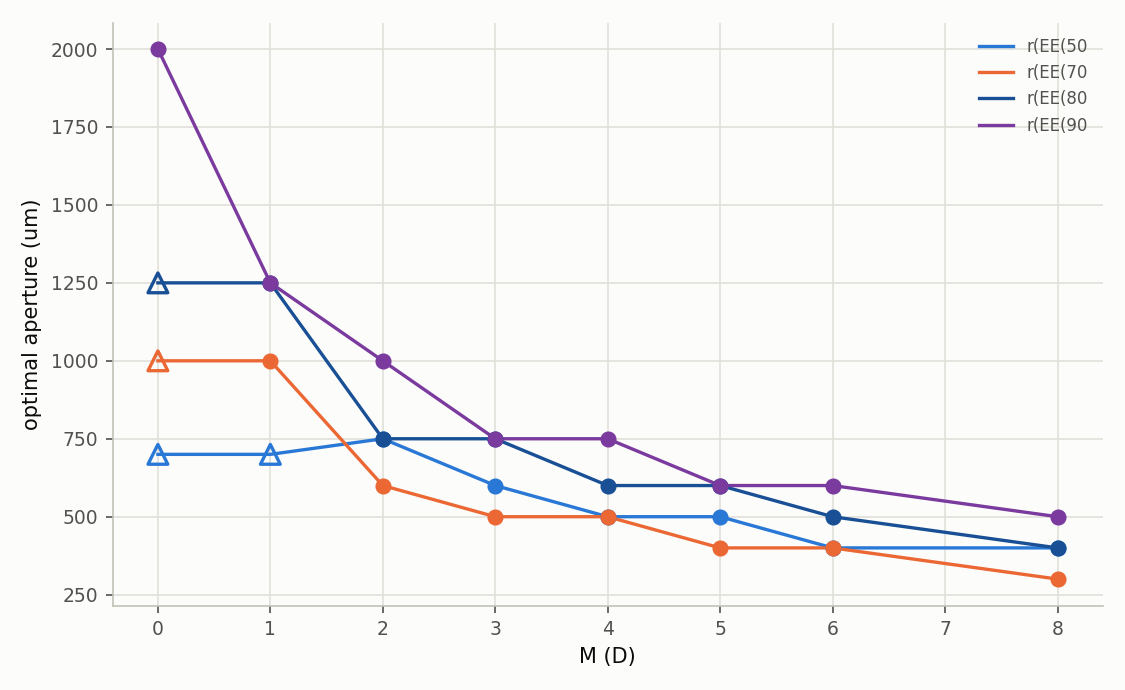
\includegraphics[width=0.85\textwidth]{figures/fig_percentile_optimum_vs_M.png}
\caption{Optimal aperture vs.\ myopia, all four percentiles; hollow markers at $M=0,1$ flag the saturated (non-unique) $r_{EE}(70\%)$/$r_{EE}(80\%)$ points.}
\label{fig:percentile-optimum}
\end{figure}

\section{Reading the genuine ($M\ge2$) rows: $r_{EE}(50\%)$ is systematically biased toward larger apertures}

For every myopia level where the comparison is trustworthy, the optimal aperture by
$r_{EE}(70\%)$ or $r_{EE}(80\%)$ is noticeably \emph{smaller} than by $r_{EE}(50\%)$:
at $M=5\,$D, $500\um$ ($r_{EE}(50\%)$) vs.\ $400\um$ ($r_{EE}(70\%)$); at $M=8\,$D,
$400\um$ vs.\ $300\um$. This is consistent with Chapter~\ref{ch:classical_model}'s
independent finding that $r_{EE}(50\%)$ overestimates real clinical blur by roughly
$7\times$ relative to FWHM: $r_{EE}(50\%)$ stops counting energy before the broader
defocus skirt --- exactly the part of the point-spread function that grows fastest
with aperture at fixed myopia --- starts to matter, so it is systematically biased
toward preferring larger apertures than a percentile that captures more of that skirt.
\textbf{Neither this report nor its source project treats any one percentile as
uniquely correct}; this chapter's purpose is to show, quantitatively, how much the
answer moves depending on which one is chosen, and to flag precisely where that
comparison is (and is not) numerically trustworthy.
